\section{Hooke's law}

\subsection*{Resources}

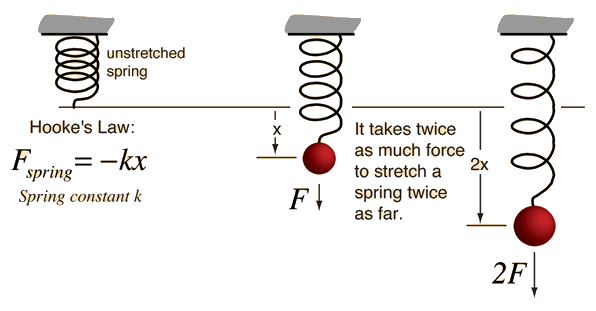
\includegraphics[scale=0.5]{hook.png}\\
\emph{(\href{http://hyperphysics.phy-astr.gsu.edu/hbase/imgmec/hook.gif}{Image} from HyperPhysics by Rod Nave, Georgia State University)}

\subsection*{Challenge}
2nd-order differential equations deal with oscillations.

Considering Hooke's law, what are $A$ and $C$ in the following equation?
\begin{equation}
    A x'' + C x = 0
\end{equation}

To check your answer, substitute a mass of \SI{2}{kg} and spring-constant of \SI{3}{kg/s^2} as appropriate.

\subsection*{Solution}
Enter only numberical values without units such as kg.

A: \hash{gg}{4e5fe6}

C: \hash{hh}{6a7015}




%%%%%%%%%%%%%%%%%%%%%%%%%%%%%%%%%
\newpage
%%%%%%%%%%%%%%%%%%%%%%%%%%%%%%%%%
\section{Exponentials and trigonometry}

\subsection*{Resources}
\begin{itemize}
    \item Text: \url{https://www.phy.duke.edu/~rgb/Class/phy51/phy51/node15.html}
\end{itemize}

\subsection*{Challenge}
Write $sin(x)$ and $cos(x)$ in exponential form.

\subsection*{Solution}

Check your answer with someone if you are unsure.


\timebox




%%%%%%%%%%%%%%%%%%%%%%%%%%%%%%%%%
\newpage
%%%%%%%%%%%%%%%%%%%%%%%%%%%%%%%%%
\section{Characteristic equation: understanding}

\subsection*{Resources}
\begin{itemize}
    \item Text: \url{http://tutorial.math.lamar.edu/getfile.aspx?file=S,88,N}
\end{itemize}

\subsection*{Comment}
A homogeneous (ie, equal to zero) second-order differential equation typically takes the form:

\begin{equation}
    A \frac{d^2y}{dt^2} + B \frac{dy}{dt} + C y = 0
\end{equation}

The first (A) term describes acceleration, while the third (C) term is the force-constant term (something like the ``stiffness'' of the spring). The second (B) term could describe a frictional force that is proportional to the velocity ($dy/dt$). Due to its relation with oscillation (and by extension, sines and cosines which can be expressed in terms of exponentials) we can typically assume an exponential-form solution to the differential equation.

\subsection*{Challenge}
Show that, assuming that all solutions to a 2nd-order differential equation of the form above will have solutions $y(t)=e^{rt}$, the value of $r$ can in principle be determined by solving the following a quadratic equation of the form
\begin{equation}
    A r^2 + Br + C = 0
\end{equation}

\subsection*{Solution}
If you are unsure of your derivation, please ask someone.

\timebox




%%%%%%%%%%%%%%%%%%%%%%%%%%%%%%%%%
\newpage
%%%%%%%%%%%%%%%%%%%%%%%%%%%%%%%%%
\section{Characteristic equation: roots}

\subsection*{Resources}
\begin{itemize}
    \item Text: \url{http://tutorial.math.lamar.edu/getfile.aspx?file=S,88,N}
\end{itemize}

\subsection*{Challenge}
Sum the points of the differential equations that have characteristic equations with
\begin{itemize}
    \item Real, distinct roots
    \item Complex roots
    \item Equal roots
\end{itemize}

1 point: $\displaystyle -3 y'' - 5 y' + 2 y = 0$ % C

2 points: $\displaystyle 3 y'' - 4 y' + 3 y = 0$ % E

4 points: $\displaystyle 3 y'' - 6 y' + 3 y = 0$ % B

8 points: $\displaystyle 3 y'' - 5 y' + 2 y = 0$ % F

16 points: $\displaystyle 3 y'' - 5 y' + 4 y = 0$ % D

32 points: $\displaystyle 3 y'' + 5 y' + 2 y = 0$ % A

\subsection*{Solution}

\begin{itemize}
    \item Real, distinct roots: \hash{ii}{064a6e}
    \item Complex roots: \hash{jj}{50385e}
    \item Equal roots: \hash{kk}{70cd8f}
\end{itemize}

\timebox




%%%%%%%%%%%%%%%%%%%%%%%%%%%%%%%%%
\newpage
%%%%%%%%%%%%%%%%%%%%%%%%%%%%%%%%%
\section{Characteristic equation: real roots with positive B}

\subsection*{Resources}
\begin{itemize}
    \item Text: \url{http://tutorial.math.lamar.edu/getfile.aspx?file=S,94,N}
\end{itemize}

\subsection*{Comment}

\subsection*{Challenge}
Solve the following 2nd-order differential equation that has real roots:

\begin{equation}
    \label{eq:ccrrpb}
    y'' + 3 y' + 2 y = 0
\end{equation}

with initial conditions $y(0)=5$ and $y'(0)=-8$.

To check your answer, substitute $t=1$ into the final expression.


\subsection*{Solution}
\hash{mm}{9b9be5}




%%%%%%%%%%%%%%%%%%%%%%%%%%%%%%%%%
\newpage
%%%%%%%%%%%%%%%%%%%%%%%%%%%%%%%%%
\section{Characteristic equation: real roots with negative B}

\subsection*{Resources}
\begin{itemize}
    \item Text: \url{http://tutorial.math.lamar.edu/getfile.aspx?file=S,94,N}
\end{itemize}

\subsection*{Challenge}
Solve the following 2nd-order differential equation that has real roots. 

\begin{equation}
    y'' - 3 y' + 2 y = 0
\end{equation}

with initial conditions $y(0)=5$ and $y'(0)=8$. Substitue $t=1$ into the final expression to check your answer.

Note that this equation is the same as equation \ref{eq:ccrrpb}, but simply the dampening (friction) term B has been changed from positive to negative.


\subsection*{Solution}
\hash{nn}{473835}

\timebox




%%%%%%%%%%%%%%%%%%%%%%%%%%%%%%%%%
\newpage
%%%%%%%%%%%%%%%%%%%%%%%%%%%%%%%%%
\section{Characteristic equation: B in equations with real roots}

\subsection*{Challenge}

\emph{(Note that there are two parts to this challenge.)}

1. Considering real root, sum the points of the following true statements:

Considering the equation

\begin{equation}
    A y'' + B y' + C y = 0
\end{equation}

1 point: Positive damping (positive B) leads to solutions with exponentials with positive exponents.

2 points: Positive damping (positive B) leads to solutions with exponentials with negative exponents.

4 points: Negative damping (negative B) leads to solutions with exponentials with positive exponents.

8 points: Negative damping (negative B) leads to solutions with exponentials with negative exponents.

16 points: Exponentials with positive exponents (eg, $e^{t}$) lead to exponential growth (instability).

32 points: Exponentials with negative exponents (eg, $e^{-t}$) lead to exponential growth (instability).

64 points: Exponentials with positive exponents (eg, $e^{t}$) lead to a damped signal (stability).

128 points: Exponentials with negative exponents (eg, $e^{-t}$) lead to damped signal (stability).

\vspace{2em}

2. Write a sentence summarising your understanding of the significance of having a positive or negative coefficient of $B$ when the roots are real.


\subsection*{Solution}
\hash{oo}{fa6adf}

\timebox




%%%%%%%%%%%%%%%%%%%%%%%%%%%%%%%%%
\newpage
%%%%%%%%%%%%%%%%%%%%%%%%%%%%%%%%%
\section{Characteristic equation: equal roots}

\subsection*{Resources}
\begin{itemize}
    \item Text: \url{http://tutorial.math.lamar.edu/getfile.aspx?file=S,96,N}
\end{itemize}

\subsection*{Comment}
It is not necessary to follow the full derivation in the suggested resource.

\subsection*{Challenge}
Solve the equation
\begin{equation}
    y'' - 2y' + y = 0
\end{equation}

To check your solution, substitute $t=1$ into the equation and assume $c_1 = c_2 = 1$.

\subsection*{Solution}
\hash{pp}{ff7ca2}

\timebox




%%%%%%%%%%%%%%%%%%%%%%%%%%%%%%%%%
\newpage
%%%%%%%%%%%%%%%%%%%%%%%%%%%%%%%%%
\section{Characteristic equation: complex roots with B=0}

\subsection*{Resources}
\begin{itemize}
    \item Text: \url{http://tutorial.math.lamar.edu/getfile.aspx?file=S,96,N}
\end{itemize}

\subsection*{Challenge}
1. Assuming there is no damping term (ie, $B=0$) show that the roots for the differential equation
\begin{equation}
    A y'' + Cy = 0
\end{equation}
are $\pm i \sqrt{C/A}$.

2. Solve the following ODE:
\begin{equation}
    \label{eq:cecr}
    y'' + 4 \pi^2 y = 0
\end{equation}

To check your answer, assume integration constants of 1 and calculate $y(\pi/2)$.

\subsection*{Solution}
Solution to part 2: \hash{qq}{7eb2c9}

\timebox




%%%%%%%%%%%%%%%%%%%%%%%%%%%%%%%%%
\newpage
%%%%%%%%%%%%%%%%%%%%%%%%%%%%%%%%%
\section{Characteristic equation: complex roots with positive B}

\subsection*{Resources}
\begin{itemize}
    \item Text: \url{http://tutorial.math.lamar.edu/getfile.aspx?file=S,96,N}
\end{itemize}

\subsection*{Challenge}
Solve the following ODE:
\begin{equation}
    y'' + y' + y = 0
\end{equation}

To check your answer, assume integration constants of 1 and calculate $y(\pi/2)$.

\subsection*{Solution}
\hash{rr}{1d0cb5}

\timebox




%%%%%%%%%%%%%%%%%%%%%%%%%%%%%%%%%
\newpage
%%%%%%%%%%%%%%%%%%%%%%%%%%%%%%%%%
\section{Characteristic equation: complex roots with negative B}

\subsection*{Resources}
\begin{itemize}
    \item Text: \url{http://tutorial.math.lamar.edu/getfile.aspx?file=S,96,N}
\end{itemize}

\subsection*{Challenge}
Solve the following ODE:
\begin{equation}
    y'' - y' + y = 0
\end{equation}

To check your answer, assume integration constants of 1 and calculate $y(\pi/2)$.

\subsection*{Solution}
\hash{ss}{caf35b}

\timebox




%%%%%%%%%%%%%%%%%%%%%%%%%%%%%%%%%
\newpage
%%%%%%%%%%%%%%%%%%%%%%%%%%%%%%%%%
\section{Damping}
\label{sec:damping}

\subsection*{Resources}
\begin{itemize}
    \item Wikipedia: https://en.wikipedia.org/wiki/Damping
\end{itemize}

\subsection*{Challenge}
Of the 6 functions shown in the graph, place the 3 that correspond to overdamped, critially damped and underdamped in the order mentioned in this sentence.

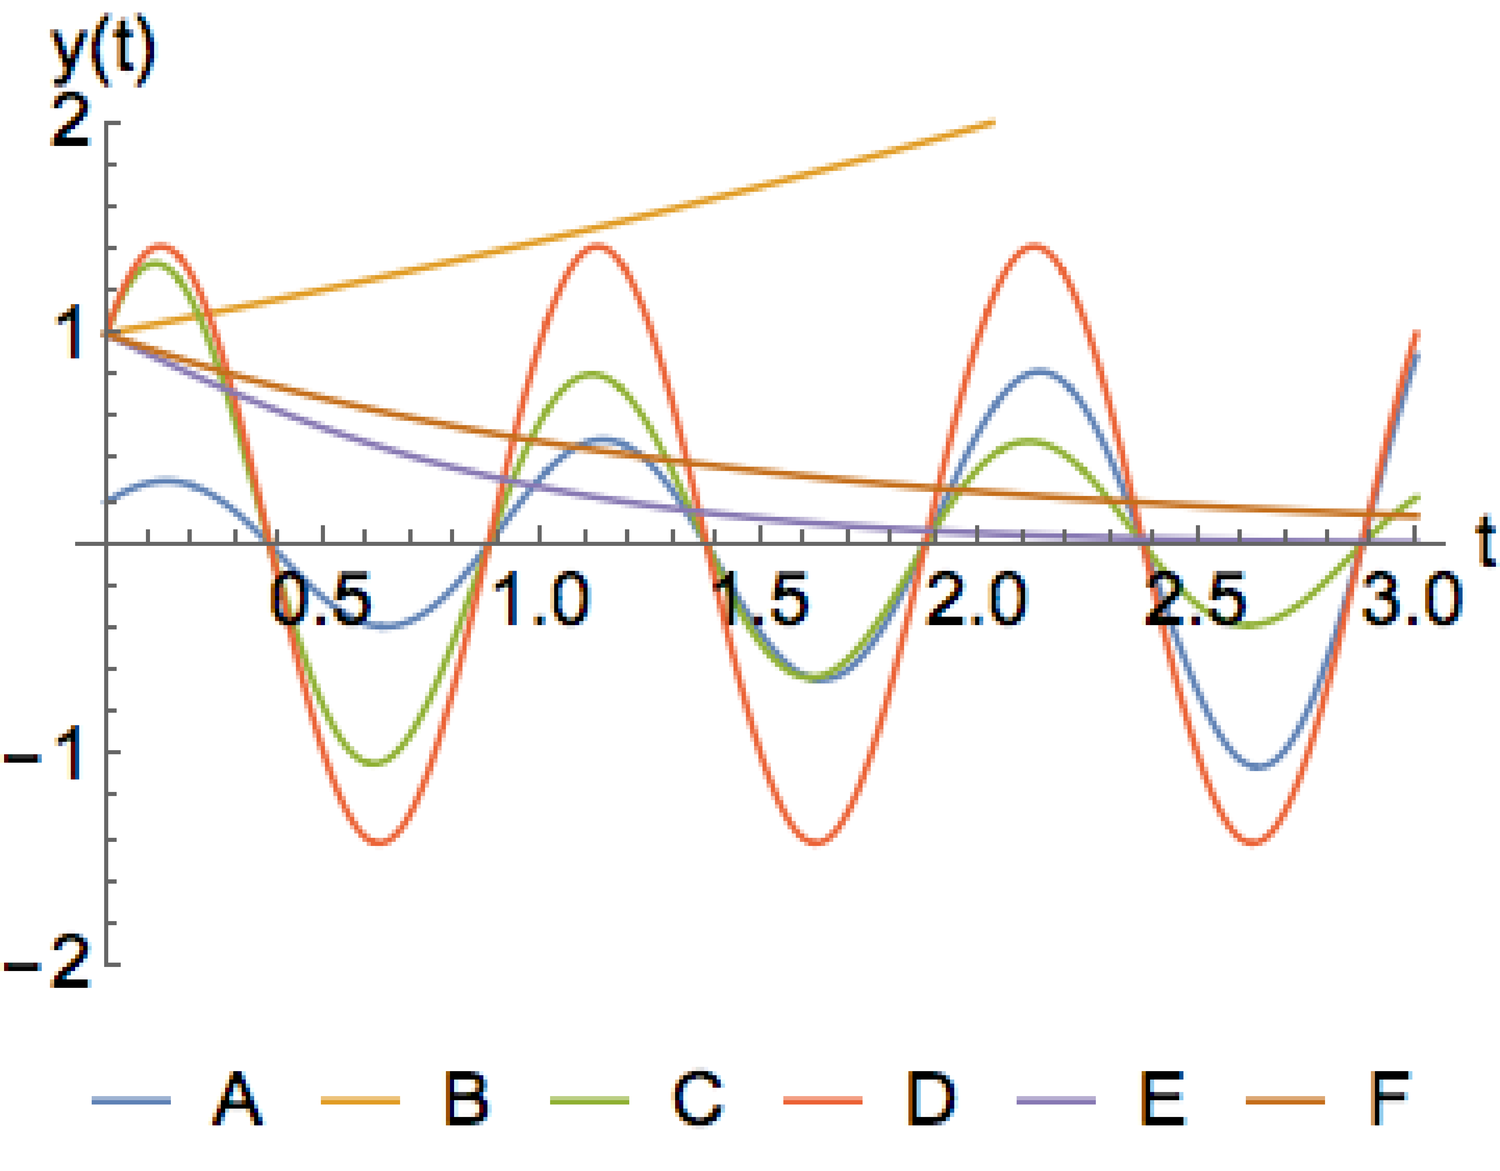
\includegraphics{damping.png}

\subsection*{Solution}
(eg, ``abc'')

\hash{tt}{060b2a}

\timebox



%%%%%%%%%%%%%%%%%%%%%%%%%%%%%%%%%
\newpage
%%%%%%%%%%%%%%%%%%%%%%%%%%%%%%%%%
\section{Damping and 2nd-order differential equations}

\subsection*{Challenge}
1. The 6 functions shown in the graph in challenge \ref{sec:damping} may represent solutions of a 2nd-order differential equation. Place the solutions A-F in the order shown below. Note that one of the descriptions below is impossible, and you should ignore that one.

I. Solution of a 2nd-order differential equation with real roots and positive B.

II. Solution of a 2nd-order differential equation with real roots and negative B.

III. Solution of a 2nd-order differential equation with real roots and B=0.

IV. Solution of a 2nd-order differential equation with equal roots.

V. Solution of a 2nd-order differential equation with complex roots and B=0.

VI. Solution of a 2nd-order differential equation with complex roots and positive B.

VII. Solution of a 2nd-order differential equation with complex roots and negative B.

\vspace{1em}
2. Write one sentence stating why one of the above solutions is impossible.

\subsection*{Solution}
(eg, ``abcdef'')

\hash{uu}{a96870}

\timebox



% One problem proving that one case is a fundamental solution
%%%%%%%%%%%%%%%%%%%%%%%%%%%%%%%%%%
%\newpage
%%%%%%%%%%%%%%%%%%%%%%%%%%%%%%%%%%
%\section{The Wronskian}
%
%\subsection*{Resources}
%\begin{itemize}
%    \item 
%\end{itemize}
%
%\subsection*{Challenge}
%Imagine you need to write a letter to a student, explaining what the Wronskian is, where it comes from, and how it is useful in determining the validity of fundamental sets of solutions. You may assume the student knows the formulas for solving different forms (complex, real and equal-roots) of 2nd-order ODE's with the characteristic equation method, but does not know what is meant by a ``fundamental solution'', doesn't understand why such fundamental solutions are sums of two terms, and does not know about the Wronskian. You may use the suggested resource to help formulate your letter. The student also would like to know about the connection of the Wronskian to linear independence and how this is related to the fundamental solutions (ie, why it matters that the two terms of the fundamental solutions are linearly independent).
%
%\emph{Suggested length: 1 A4 sheet.}
%
%\subsection*{Solution}
%Please give the letter to the teacher for posting. The teacher will check the depth of your understanding prior to posting.
%
%\timebox




%%%%%%%%%%%%%%%%%%%%%%%%%%%%%%%%%
%\newpage
%%%%%%%%%%%%%%%%%%%%%%%%%%%%%%%%%
%\section{Characteristic equation: exersizes}

%\subsection*{Challenge}
%Solve the following 2nd-order differential equations:

%\begin{equation}
    
%\end{equation}

%\subsection*{Solution}
%(eg, ``abcdef'')

%\hash{uu}{a96870}

%\timebox
